\documentclass[10pt,a4paper]{article}
\usepackage[utf8]{inputenc}
\usepackage{amsmath}
\usepackage{amsfonts}
\usepackage{amssymb}
\usepackage{graphicx}
\usepackage{verbatim}
\usepackage[margin=1in]{geometry}
\usepackage{listings} % for formatting code
\lstset
{
    language=C,
    basicstyle=\footnotesize\ttfamily,
    numbers=left,
    stepnumber=1,
    showstringspaces=false,
    tabsize=1,
    breaklines=true,
    breakatwhitespace=false,
}

\setlength\parindent{0pt} % Removes all indentation from paragraphs

\author{Nikola Janju\v{s}evi\'{c}}
\title{ECE357, Computer Operating Systems -- Problem Set \#2, Problem 3}

\begin{document}
\begin{Large}
ECE357, Computer Operating Systems -- Problem Set \#2, Problem 3
\end{Large} \\
\begin{large}
Nikola Janju\v{s}evi\'{c}
\end{large} 
\\
\today

\section*{Example Usage}
\begin{figure}[h]
	\centering
	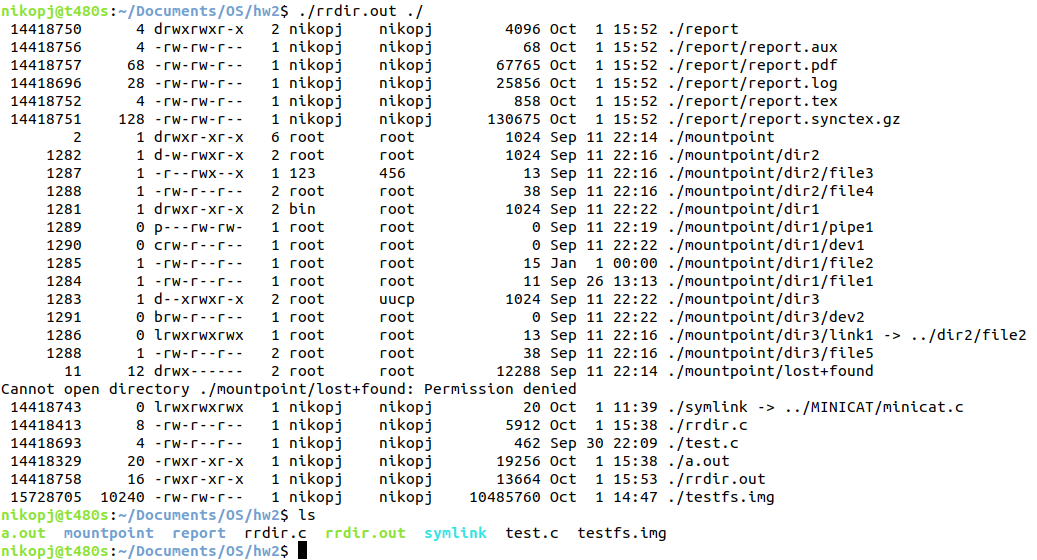
\includegraphics[width=\textwidth]{currentwd_ss2.png}
\end{figure}

\pagebreak
\section*{Program: \texttt{rrdir.c}}

\lstinputlisting[language=C]{../rrdir.c}

\end{document}